\section{Obtaining perfect proper (2,3)-poles}\label{sec:classes-to-perfect}

It may be convenient to modify some proper (2,3)-poles by adding some vertices and edges to obtain perfect proper (2,3)-pole. If we know in which colouring class the proper (2,3)-pole is, then we can make a junction with the specific constructions provided in this chapter to obtain perfect colouring, of course, only if the former (2,3)-pole is colourable. 

\subsection{Extending class 1A to 2B}

Let $T(A,B)$ be a proper (2,3)-pole, whose colouring class is 1A and let it allow a solitary cycle $b_ia_1a_2$ for some $b_i\in B$. Now let $T'(A,B')$, $B'=(b'_1, b'_2, b'_3)$ be a proper (2,3)-pole obtained by the partial junction of $T$ with the 6-pole $M$ shown in \cref{fig:1A2B}. In this partial junction we connect the connector $B$ and the connector $(c_1,c_2,c_3)$ such that it contains a junction of $b_i$ and $c_1$. We prove that the result is a proper (2,3)-pole from colouring class 2B, which allows solitary cycle $b'_2a_1b'_3a_2$.

\begin{proof}
	Without loss of generality, let the semiedge $b_i$ be $b_1$. Let this colouring of $T$ be $\phi$. Using a colouring $\phi_1$ of $M$ where $\phi_1(b'_1,b'_2,b'_3)=(3,3,2)$ and a colouring $\phi_2$ of $M$ where $\phi_2(b'_1,b'_2,b'_3)=(3,2,3)$, in both cases $\phi_1(c_1,c_2,c_3)=\phi_2(c_1,c_2,c_3)=(2,1,1)$. After the mentioned partial junction of $T$ and $M$, we can colour the rest of $T'$ by the~colouring $\phi$. We can see that the colouring graph of $T'$ allows a solitary cycle $b'_2a_1b'_3a_2$. No more colourings can be obtained since, as it can be seen, $b'_2$ and $b'_3$ must have different colours, so one of them is always solitary and we cannot obtain classes $2A,3B$, and perfect.
\end{proof}

\begin{figure}
	\centering
	\scalebox{0.7}{
		%\begin{tikzpicture}[every node/.style={draw,circle,very thick, fill=black}]
%	
%	\node[draw=none, fill=none] (1) at (-1,2) {$c_1$};
%	\node[draw=none, fill=none] (2) at (-1,1) {$c_2$};
%	\node[draw=none, fill=none] (3) at (-1,0) {$c_3$};
%	\node (4) at (1,2) {};
%	\node (5) at (1,1) {};
%	\node (6) at (1,0) {};
%	\node (7) at (2,2) {};
%	\node[draw=none, fill=none] (9) at (4,2.5) {$b'_1$};
%	\node[draw=none, fill=none] (10) at (4,1.5) {$b'_2$};
%	\node[draw=none, fill=none] (11) at (4,0) {$b'_3$};
%	
%	\path (1) edge (4);
%	\path (2) edge (5);
%	\path (3) edge (6);
%	\path (4) edge (5);
%	\path (5) edge (6);
%	\path (4) edge (7);
%	\path (7) edge (9);
%	\path (7) edge (10);
%	\path (6) edge (11);
%	
%\end{tikzpicture}

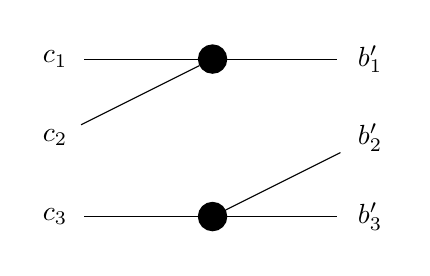
\begin{tikzpicture}[every node/.style={draw,circle,very thick, fill=black}]
	
	\node[draw=none, fill=none] (1) at (-1,2) {$c_1$};
	\node[draw=none, fill=none] (2) at (-1,1) {$c_2$};
	\node[draw=none, fill=none] (3) at (-1,0) {$c_3$};
	\node (4) at (1,2) {};
	\node (5) at (1,0) {};
	\node[draw=none, fill=none] (6) at (3,2) {$b'_1$};
	\node[draw=none, fill=none] (7) at (3,1) {$b'_2$};
	\node[draw=none, fill=none] (8) at (3,0) {$b'_3$};
	
	\path (1) edge (4);
	\path (2) edge (4);
	\path (3) edge (5);
	\path (4) edge (6);
	\path (5) edge (7);
	\path (5) edge (8);
	
\end{tikzpicture}
	}
	\caption{6-pole used to create colouring class 2B from 1A}
	\label{fig:1A2B}
\end{figure}

%\begin{figure*}
%	\centering
%	\begin{subfigure}{0.49\textwidth}
%		\centering
%		%\begin{tikzpicture}[every node/.style={draw,circle,very thick, fill=black}]
%	
%	\node[draw=none, fill=none] (1) at (-1,2) {$c_1$};
%	\node[draw=none, fill=none] (2) at (-1,1) {$c_2$};
%	\node[draw=none, fill=none] (3) at (-1,0) {$c_3$};
%	\node (4) at (1,2) {};
%	\node (5) at (1,1) {};
%	\node (6) at (1,0) {};
%	\node (7) at (2,2) {};
%	\node[draw=none, fill=none] (9) at (4,2.5) {$b'_1$};
%	\node[draw=none, fill=none] (10) at (4,1.5) {$b'_2$};
%	\node[draw=none, fill=none] (11) at (4,0) {$b'_3$};
%	
%	\path (1) edge node[draw=none, fill=none,above] {3} (4);
%	\path (2) edge node[draw=none, fill=none,above] {3} (5);
%	\path (3) edge node[draw=none, fill=none,above] {3} (6);
%	\path (4) edge node[draw=none, fill=none,right] {2} (5);
%	\path (5) edge node[draw=none, fill=none,right] {1} (6);
%	\path (4) edge node[draw=none, fill=none,above] {1} (7);
%	\path (6) edge node[draw=none, fill=none,above] {2} (11);
%	\path (7) edge node[draw=none, fill=none,above] {3} (9);
%	\path (7) edge node[draw=none, fill=none,below] {2} (10);
%	
%\end{tikzpicture}

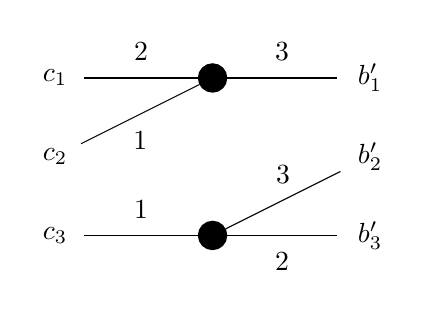
\begin{tikzpicture}[every node/.style={draw,circle,very thick, fill=black}]
	
	\node[draw=none, fill=none] (1) at (-1,2) {$c_1$};
	\node[draw=none, fill=none] (2) at (-1,1) {$c_2$};
	\node[draw=none, fill=none] (3) at (-1,0) {$c_3$};
	\node (4) at (1,2) {};
	\node (5) at (1,0) {};
	\node[draw=none, fill=none] (6) at (3,2) {$b'_1$};
	\node[draw=none, fill=none] (7) at (3,1) {$b'_2$};
	\node[draw=none, fill=none] (8) at (3,0) {$b'_3$};
	
	\path (1) edge node[draw=none, fill=none,above] {2} (4);
	\path (2) edge node[draw=none, fill=none,below] {1} (4);
	\path (3) edge node[draw=none, fill=none,above] {1} (5);
	\path (4) edge node[draw=none, fill=none,above] {3} (6);
	\path (5) edge node[draw=none, fill=none,above] {3} (7);
	\path (5) edge node[draw=none, fill=none,below] {2} (8);
	
\end{tikzpicture}
%	\end{subfigure}
%	\hfill
%	\begin{subfigure}{0.49\textwidth}
%		\centering
%		%\begin{tikzpicture}[every node/.style={draw,circle,very thick, fill=black}]
%	
%	\node[draw=none, fill=none] (1) at (-1,2) {$c_1$};
%	\node[draw=none, fill=none] (2) at (-1,1) {$c_2$};
%	\node[draw=none, fill=none] (3) at (-1,0) {$c_3$};
%	\node (4) at (1,2) {};
%	\node (5) at (1,1) {};
%	\node (6) at (1,0) {};
%	\node (7) at (2,2) {};
%	\node[draw=none, fill=none] (9) at (4,2.5) {$b'_1$};
%	\node[draw=none, fill=none] (10) at (4,1.5) {$b'_2$};
%	\node[draw=none, fill=none] (11) at (4,0) {$b'_3$};
%	
%	\path (1) edge node[draw=none, fill=none,above] {3} (4);
%	\path (2) edge node[draw=none, fill=none,above] {3} (5);
%	\path (3) edge node[draw=none, fill=none,above] {3} (6);
%	\path (4) edge node[draw=none, fill=none,right] {2} (5);
%	\path (5) edge node[draw=none, fill=none,right] {1} (6);
%	\path (4) edge node[draw=none, fill=none,above] {1} (7);
%	\path (6) edge node[draw=none, fill=none,above] {2} (11);
%	\path (7) edge node[draw=none, fill=none,above] {2} (9);
%	\path (7) edge node[draw=none, fill=none,below] {3} (10);
%	
%\end{tikzpicture}

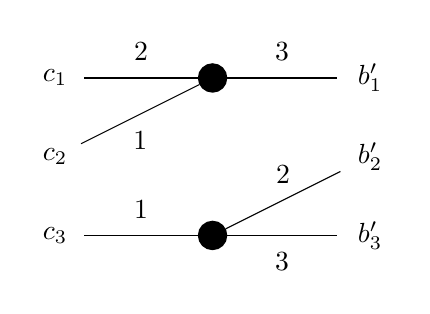
\begin{tikzpicture}[every node/.style={draw,circle,very thick, fill=black}]
	
	\node[draw=none, fill=none] (1) at (-1,2) {$c_1$};
	\node[draw=none, fill=none] (2) at (-1,1) {$c_2$};
	\node[draw=none, fill=none] (3) at (-1,0) {$c_3$};
	\node (4) at (1,2) {};
	\node (5) at (1,0) {};
	\node[draw=none, fill=none] (6) at (3,2) {$b'_1$};
	\node[draw=none, fill=none] (7) at (3,1) {$b'_2$};
	\node[draw=none, fill=none] (8) at (3,0) {$b'_3$};
	
	\path (1) edge node[draw=none, fill=none,above] {2} (4);
	\path (2) edge node[draw=none, fill=none,below] {1} (4);
	\path (3) edge node[draw=none, fill=none,above] {1} (5);
	\path (4) edge node[draw=none, fill=none,above] {3} (6);
	\path (5) edge node[draw=none, fill=none,above] {2} (7);
	\path (5) edge node[draw=none, fill=none,below] {3} (8);
	
\end{tikzpicture}
%	\end{subfigure}
%	\caption{Colourings of the 6-pole used to extend class 1A to 2B}
%	\label{fig:1A2BCol}
%\end{figure*}

It is the smallest such 6-pole, considering the number of vertices, which extends class 1A to 2B.

\subsection{Extending class 2B to 2A}

Let $T(A,B)$ be a proper (2,3)-pole whose colouring class is 2B. Let $b_i,b_j,i\neq j$ be the two semiedges from $B$, for which there exists a solitary cycle $a_1b_ia_2b_j$. Now let $T'(A,B')$, $B'=(b'_1, b'_2, b'_3)$ be a proper (2,3)-pole obtained by the partial junction of $T$ with the 6-pole on \cref{fig:multiple} by the junction of semiedges $b_i$ to $c_1$, $b_j$ to $c_2$ and the last semiedge to $c_3$. The result $T'$ is from a colouring class $2A$ and allows solitary cycle $a_1b'_1a_2b'_2a_1$. The proof is similar to the one in extending class 1A to 2B.

%\begin{proof}
%	Without loss of generality, let $b_i,b_j$ be $b_1,b_2$ respectively. Let us denote the structure in  \cref{fig:multiple} as $M$. If we order the semiedges of $M$ as $(c_1,c_2,c_3,b'_1,b'_2,b'_3)$, we see that its colouring set contains among others the colourings $(2,1,1,2,1,1), (1,2,1,1,2,1), \newline (2,1,1,2,2,2)$, thus after the mentioned junction we can colour the result in a way that the solitary cycle will be $a_1b'_1a_2a_1b'_2a_2$.
%	
%	Let's say we would want the solitary cycle of the result to contain $b'_3$ as well, in a colouring $\phi$. This would mean that $\phi(b'_1)=\phi(b'_2)$, and both are not equal to $\phi(b'_3)$. However, as it can be checked, the colours of the resulting semiedges would be unambiguously set as $\phi(c_1)=\phi(c_2)=\phi(b'_1)=\phi(b'_2)$ and $\phi(c_3)=\phi(b'_3)$. Since we perform the junction as explained above, $b_3$ has to be contained in the solitary cycle of $T(A,B)$, which is false. This means that we can't obtain the class 3B nor the perfect colouring.
%\end{proof}

\begin{figure}[h]
	\centering
	\scalebox{0.7}{
		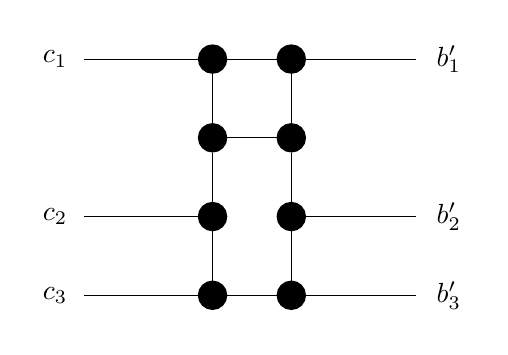
\begin{tikzpicture}[every node/.style={draw,circle,very thick, fill=black}]
	
	\node[draw=none, fill=none] (1) at (-1,3) {$c_1$};
	\node[draw=none, fill=none] (2) at (-1,1) {$c_2$};
	\node[draw=none, fill=none] (3) at (-1,0) {$c_3$};
	\node (4) at (1,3) {};
	\node (5) at (1,2) {};
	\node (6) at (1,1) {};
	\node (7) at (1,0) {};
	\node (8) at (2,3) {};
	\node (9) at (2,2) {};
	\node (10) at (2,1) {};
	\node (11) at (2,0) {};
	\node[draw=none, fill=none] (12) at (4,3) {$b'_1$};
	\node[draw=none, fill=none] (13) at (4,1) {$b'_2$};
	\node[draw=none, fill=none] (14) at (4,0) {$b'_3$};
	
	\path (1) edge (4);
	\path (2) edge (6);
	\path (3) edge (7);
	\path (4) edge (5);
	\path (5) edge (6);
	\path (6) edge (7);
	
	\path (8) edge (9);
	\path (9) edge (10);
	\path (10) edge (11);
	
	\path (8) edge (12);
	\path (10) edge (13);
	\path (11) edge (14);
	
	\path (4) edge (8);
	\path (5) edge (9);
	\path (7) edge (11);

\end{tikzpicture}
	}
	\caption{6-pole used to extend multiple colouring classes}
	\label{fig:multiple}
\end{figure}

It must be noted that this construction produces proper (2,3)-poles which may not be contained in a nontrivial snark, since it contains a quadrilateral. If we would need to extend some proper (2,3)-pole to obtain a specific colouring class and require the~extended proper (2,3)-pole to be contained in a nontrivial snark, we would need to use other, more complex constructions.

\subsection{Extending proper (2,3)-poles from class 2A to perfect}

To extend a proper (2,3)-pole from the colouring class 2A to a perfect one, the same 6-pole can be used as before, just with a different junction. Let $T(A,B)$ be a proper (2,3)-pole whose colouring class is 2B. Let $b_i,b_j,i\neq j$ be the two semiedges from $B$, for which there exists a solitary cycle $a_1b_ia_2a_1b_ja_2$. Now let $T'(A,B')$, $B'=\{b'_1, b'_2, b'_3\}$ be a proper (2,3)-pole obtained by the junction of $T$ with the 6-pole in \cref{fig:multiple} by the~junction of semiedges $b_i$ to $c_2$, $b_j$ to $c_3$ and the last semiedge to $c_1$. The result $T'$ is a~perfect proper (2,3)-pole, which can be proved similarly to before.

%\begin{proof}
%	Let $b_i,b_j$ be $b_1,b_2$ respectively, so in the junction we connect $b_1$ to $c_2$ and $b_2$ to $c_3$. Let us denote the structure in  \cref{fig:multiple} as $M$. If we order the semiedges of $M$ as $(c_1,c_2,c_3,b'_1,b'_2,b'_3)$, we see that its colouring set contains the colourings $(2,1,2,1,2,2), (2,1,2,2,1,2), (2,2,1,2,2,1), (2,2,2,2,2,2)$, thus after the mentioned junction we can colour the result in a way that it will be perfect.
%\end{proof}

\subsection{Extending proper (2,3)-poles from class 3B to perfect}

Let $T(A,B)$ be a proper (2,3)-pole whose colouring class is 3B. Let $T'(A,B')$, \linebreak ${B'=(b'_1, b'_2, b'_3)}$ be a proper (2,3)-pole obtained by the partial junction of $T$ with the 6-pole on \cref{fig:multiple}, performing the junction of $B$ to $(c_1,c_2,c_3)$. Then $T'$ is perfect, which can be proved similarly to before.

%\begin{proof} 
%	Let us denote the structure in  \cref{fig:multiple} as $M$. If we order the semiedges of $M$ as $(c_1,c_2,c_3,b'_1,b'_2,b'_3)$, we see that its colouring set contains the colourings $(2,1,2,1,2,2), (2,1,2,2,1,2), (2,2,1,2,2,1), (2,1,1,2,2,2)$, thus after the mentioned junction we can colour the result in a way that it will be perfect.
%\end{proof}

It is possible to incrementally modify each colourable proper (2,3)-pole to obtain a perfect one. For example, from class 1A it is possible to get class 2B, then 2A and finally perfect. It is evident that extending uncolourable multipoles to obtain colourable is impossible.